% ********** Chapter 1 **********
\section{Analyse}
\label{sec:chap1:ana}

In diesem Abschnitt wird erl"autert wie der erste Teil der Aufgabenstellung analysiert wurde, welche Use-Cases dabei gefunden 
wurden, und wie aus diesen Use-Cases Arbeitspakete abgeleitet wurden. Dieser erste Teil umfasste haupts"achlich das Ausf"uhren 
von PHP-Sourcecode innerhalb einer Java-Anwendung. 
Die Anforderung war m"oglichst grosse Teile des XP-Frameworks innerhalb von Java auszuf"uhren.
Vom vollen Umfang des XP-Frameworks ausgenommen waren lediglich die Komponenten welche eine Kommunikation
nach aussen erlaubten, so zum Beispiel die Datenbankkonnektivit"at, da diese Funktionen sp"ater vom Application Server
bereitgestellt werden sollten. Idealerweise sollte die verwendete PHP Version leicht austauschbar sein. Eine weitere
Anforderung war die Interaktion von Java nach PHP und umgekehrt m"oglichst einfach zu gestalten, Java-Objekte sollen
in PHP erzeug- und zugreifbar sein.

\subsection{Use-Cases}
\label{sec:chap1:ana:uc}

Use-Cases (auch Anwendungsf"alle) definieren die Interaktion zwischen Akteuren und dem zu entwerfenden Softwaresystem.
Das Erstellen der Use-Cases soll nicht nur zu einem Besseren Verst"andnis der zu implementierenden Abl"aufe, sondern
zu einem besseren Verst"andnis der gesammten Aufgabe f"uhren. Zun"achst mussten allerdings die m"oglichen Akteure ermittelt
werden, und es ergab sich dass lediglich zwei unterschiedliche Akteure existieren: der Java-Anwender, der eine Java-Applikation
benutzt beziehungsweise entwickelt und den PHP-Anwender, dessen PHP-Skript aus Java heraus ausgef"uhrt wird. Auf oberster Ebene
wollen diese beiden Akteure Daten austauschen, beziehungsweise auf Eingaben des einen reagieren um Ergebnisse zur"uckzuliefern,
bei genauerer Betrachtung lie\ss en sich im Wesentlichen vier Use-Cases aus der Aufgabe ableiten:

\begin{figure}[h]
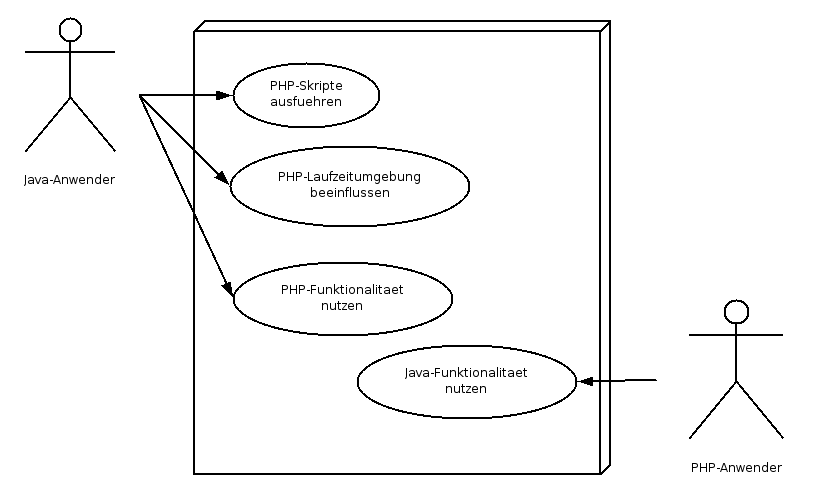
\includegraphics[width=\textwidth]{chap1/img/usecases.png}
\caption{Use-Cases}
\label{fig:usecases}
\end{figure}

\begin{description}
    \item[UC.01 - Ausf"uhren von PHP-Skripten] Ein Java-Anwender m"ochte ein oder mehrere PHP-Skripte aus einer
        Java-Applikation heraus ausf"uhren. Hierbei soll es m"oglich sein das Skript zur Laufzeit der Java-Applikation
        zu ver"andern und erneut auszuf"uhren. Weiterhin sollen Daten sowohl aus Java an das PHP-Skript "ubergeben, als
        auch Ergebnisse des Skriptes an Java zur"uck"ubergeben werden.
    \item[UC.02 - Beeinflussen der PHP Laufzeitumgebung] Es soll dem Java-Anwender m"oglich sein Einfluss auf die PHP-Laufzeitumgebung
        zu nehmen. Dies geschieht bei PHP typischerweise durch das Setzen von Initialisierungsparametern, entweder Systemweit
        in der Datei "'php.ini"', beim Starten des PHP-Interpreters, oder zur Laufzeit des PHP-Skriptes.
    \item[UC.03 - Zugriff auf Java aus PHP] Dem Entwickler eines PHP-Skriptes soll Zugriff auf m"oglichst den kompletten 
        Funktionalit"atsumfang der Java-Umgebung gew"ahrt werden. Das umfasst vor allem das Instanziieren von Java-Objekten und
        den Zugriff auf deren Methoden und Attribute, aber auch weitere Sprachfunktionen wie beispielsweise das Werfen und 
        Fangen von Exceptions. Zus"atzlich soll der Zugriff auf Java f"ur den PHP-Anwender m"oglichst intuitiv ablaufen, im
        Idealfall sollen sich Java-Objekte in PHP genauso behandeln lassen wie native PHP-Objekte.
    \item[UC.04 - Zugriff auf PHP aus Java] Es soll einem Java-Entwickler erm"oglicht werden auf einfach Art und Weise auf
        innerhalb eines PHP-Skriptes vorhandene Funktionen, Klassen und deren Methoden zuzugreiffen. Auch hier soll
        dieser Zugriff m"oglichst intuitiv erfolgen, PHP-Objekte sollen sich wie Java-Objekte benutzen lassen. 
\end{description}

\subsection{Anforderungen}
\label{sec:chap1:ana:ap}

Nachdem die Use-Cases bekannt waren musste festgelegt werden welche Einzelanforderungen sie jeweils an das System stellen.
Im Gegensatz zu den Use-Cases, die die Sicht des Anwenders auf das System darstellen, sollte dieser Schritt der Analyse
die n"otigen Funktionen ergeben, die das System bereitstellen muss, um die Anforderungen des Anwenders zu erf"ullen.
Weiterhin soll f"ur jede dieser Anforderungen beschrieben werden, wie ein Test aussehen k"onnte der ermittelt, ob die 
Anforderung erf"ullt ist.

\begin{enumerate}
\item Die PHP-ScriptEngine muss f"ur den Anwender verf"ugbar sein. Die aktuelle Java-Umgebung muss so konfiguriert sein,
    dass die PHP-ScriptEngine vom ScriptEngineManager "uber die in \ref{sec:javanscripts:jsr} beschriebenen Auffindungsmechanismen
    gefunden und instaziiert werden kann. Diese Anforderung ist eigentlich Grundlage des kompletten Systems, streng genommen wird sie
    aber nur von \emph{UC.01} gestellt.
    \textbf{Test}: Durch einfache Ausgabe auf der Konsole soll schnell ermittelbar sein, welche ScriptEngines geladen und einsatzbereit sind.

\item "Ubersetzen von PHP-Quelltext. Dem System "ubergebener PHP-Quelltext soll Gem"a\ss des in \texttt{javax.script} vorhandenen 
    Interfaces \texttt{Compilable} in eine ausf"uhrbare Form "ubersetzt werden. Das Ergebnis eines solchen "Ubersetzungsvorganges
    soll mehrfach ausgef"uhrt werden k"onnen.Beim "Ubersetzen auftretende syntaktische oder semantische Fehler sollen dem Anwender 
    als Java-Exception zur"uckgegeben werden.
    Auche diese Anforderung ist eine Vorraussetzung fast aller weiterer Anforderungen, weswegen sie ebenfalls \emph{UC.01} zugeordnet wird.
    \textbf{Test}: die "Ubergabe fehlerhaften PHP-Quelltextes soll zu einer Java-Exception f"uhren.

\item Ausf"uhren beliebiger PHP-Skripte. Es soll dem Anwender m"oglich sein, beliebige PHP-Skripte auszuf"uhren. Diese Skripte sollen
    in vielfacher Form an das System "ubergeben werden k"onnen, auch ohne dass der Anwender selbst Java-Quelltext schreiben muss.
    Zur Laufzeit des PHP-Skriptes auftretende Fehler sollen ebenfalls als Java-Exception an den Anwender weitergereicht werden.
    Aufbauend auf die beiden vorherigen Anforderungen realisiert diese Anforderung die in \emph{UC.01} geforderte Funktion.
    \textbf{Test}: Es soll auf der Kommandozeile der Name einer Datei "ubergeben werden, deren Inhalt als PHP-Skript ausgef"uhrt wird.

\item Datenaustausch. Zwischen den beiden Programmiersprachen soll der Austausch beliebiger Daten m"oglich sein. Simple (skalare)
    Datentypen sollen in ihre jeweilige Entsprechung in der anderen Sprache umgewandelt werden, komplexe Datentypen sollen in der anderen 
    Sprache als Referenz verf"ugbar sein. Auch die Daten"ubergabe mittels des vom JSR 223 definierten ScriptContext soll m"oglich sein.
    Sowohl \emph{UC.03} als auch \emph{UC.04} stellen diese Anforderung. 
    \textbf{Test}: Ein Mittels des Kontextes "ubergenes Java-Objekt soll in PHP ver"andert werden, und diese "Anderungen sollen in
    Java ausgelesen werden.

\item Erzeugen von Java-Objekten. Innerhalb eines ausgef"uhrten PHP-Skriptes soll es m"oglich sein Java-Objekte zu erzeugen und auf
    deren Methoden und Attribute zuzugreiffen. Dieser Zugriff soll f"ur den PHP-Anwnder m"oglichst einfach und intuitiv m"oglich sein.
    Diese Anforderung ist ein wesentlicher Teil von \emph{UC.03}.
    \textbf{Test}: Es soll ein Skript aufgerufen werden, welches ein Java-Objekt erzeugt, eine Methode dieses Objektes aufruft und
    deren Ergebnis an die Java-Applikation zur"uckgibt.

\item Java-Exceptions. Neben dem Zugriff auf Java-Objekte soll es dem PHP-Anwender auch m"oglich sein aus einem
    PHP-Skript heraus beliebige Java-Exceptions zu werfen. Diese Exceptions sollen entweder wie andere Java-Objekte auch vor dem Werfen,
    oder beim Werfen selbst aus einem "ubergebenen Klassennamen erzeugt werden. Dem PHP-Anwender soll ebenfalls erm"oglicht werden
    zu "uberpr"ufen ob Java-Exceptions aufgetreten sind, und aufgetretene Java-Exceptions abzuarbeiten.
    Diese Anforderung wird explizit vom \emph{UC.03} gestellt.
    \textbf{Test}: Es soll ein PHP-Skript ausgef"uhrt werden das eine Java-Exception provoziert, und auf diese Exception reagiert.

\item Weitere Java-Funktionalit"at. Implizit fordert \emph{UC.03} ebenfalls dass das System dem PHP-Anwender erlaubt grundlegende
    Funktionalit"at der Java-Umgebung zu nutzen, so soll er "uberpru"ufen k"onnen ob ein Java-Objekt identisch mit einem anderen ist
    (\ident(equals()), ob es Instanz einer bestimmten Klasse ist (\texttt{instanceof}), oder ob es sicher auf eine andere Klasse castbar ist.
    \textbf{Test}: Innerhalb eines PHP-Skriptes sollen auf einem Java-Objekt jeweils die oben genannten Tests durchgef"uhrt werden.

\item Aufrufen von Methoden in "ubersetzten Skripten. Das zu entwickelnde Softwaresystem soll das Aufrufen sowohl von globalen Funktionen,
    als auch von Objektmethoden in "ubersetzten PHP-Skripten aus Java heraus erlauben, hierzu soll das Interface \texttt{javax.script.Invocable} 
    implementiert werden. Die "Ubergebenen Funktions- und Methodenargumente sollen wie schon beim Datenaustausch in ihre PHP-Entsprechungen
    umgewandelt werden. Diese Anforderung stellt einen wesentlichen Teil des \emph{UC.04} dar.
    \textbf{Test}: Es soll aus einer Java-Applikation heraus eine PHP-Funktion aufgerufen werden die ein PHP-Objekt zur"uckgibt, welches
    ein Java-Interface implementiert. Auf diesem Objekt soll dann eine Interface-Methode aufgerufen werden.

\item Setzen von php.ini Parametern. Dem Anwender soll die M"oglichkeit geboten werden gezielt php.ini Werte zu setzen oder zu verwenden,
    um das Laufzeitverhalten von PHP wie gewohnt zu beeinflussen. Diese Werte sollen aus den Java-Systemproperties ausgelesen werden,
    da diese sowohl zur Laufzeit der Java-Applikation programmatisch als auch vor dem Start der Java-VM beispielsweise "uber die Kommandozeile
    gesetzt werden k"onnen. Die php.ini ist der gew"ohnliche Weg das Laufzeitverhalten des PHP-Interpreters zu ver"andern, somit werden
    die Anforderungen die der  \emph{UC.02} stellt komplett erf"ullt.
    \textbf{Test}: Es soll der Wert php.ini-Wert \texttt{include\_path} "uber die Kommandozeile gesetzt und in einem
    PHP-Skript ausgelesen werden. 

\end{enumerate}

Nat"urlich decken die oben aufgelisteten Anforderungen nur die grundlegende Funktionalit"at des Systems ab, im Lauf der Implementierung werden
noch weitere notwendige oder auch nur n"utzliche Funktionen gefunden und realisiert werden.
% ********** End of chapter **********
